% Appendix A
\chapter{TEST CASES}
\section{TEST CASES FOR ERROR LEVEL ANALYSIS}
In the data pre-processing module, error level analysis shows the difference in the quality level of the image when it is resaved and also the error potential. 
\subsection{TESTCASES}
\subsubsection{Authentic image}
Authentic image with a minimum difference of 4
  \begin{figure}[htp]
\centering
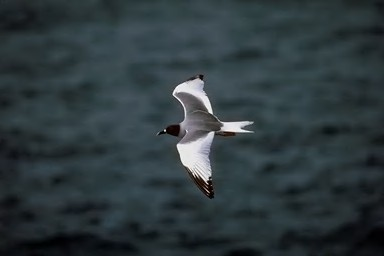
\includegraphics[width=10cm]{Figures/2.jpg}
\caption{Authentic Input image}
\label{fig:lion}
\end{figure}

\begin{figure}[htp]
\centering
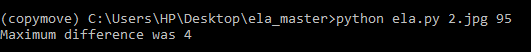
\includegraphics[width=15cm]{Figures/as.PNG}
\caption{Error displayed}
\label{fig:lion}
\end{figure}

\begin{figure}[htp]
\centering
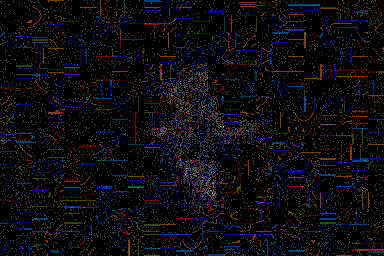
\includegraphics[width=10cm,height=6cm]{Figures/2_ela.png}
\caption{Output ELA image}
\label{fig:lion}
\end{figure}


\subsubsection{Fake image}
     The fake image with a maximum difference of 29 and its ELA image is shown.
\begin{figure}[h!]
\centering
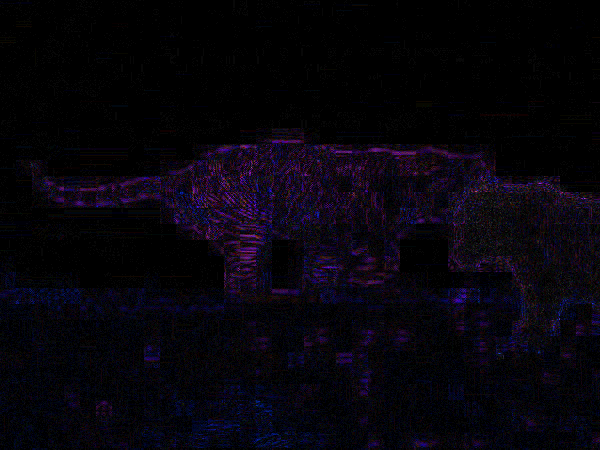
\includegraphics[width=10cm,height=6cm]{Figures/tiger_ela.png}
\caption{ELA image}
\label{fig:lion}
\end{figure}
     
\begin{figure}[h!]
\centering
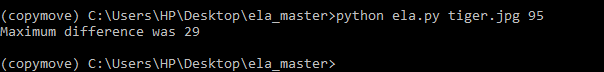
\includegraphics[width=16cm]{Figures/ela-cmd.PNG}
\caption{Error}
\label{fig:lion}
\end{figure}
\newpage

\section{OVERALL TESTCASES FOR THE SYSTEM}

\subsection{TESTCASE 1}
\subsubsection{Authentic image}
\begin{figure}[htp]
\centering
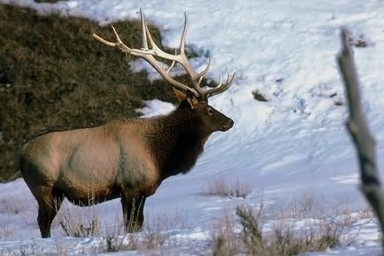
\includegraphics[width=13cm]{Figures/Au_ani_00021.jpg}
\caption{Authentic input image}
\label{fig:lion}
\end{figure}

\begin{figure}[htp]
\centering
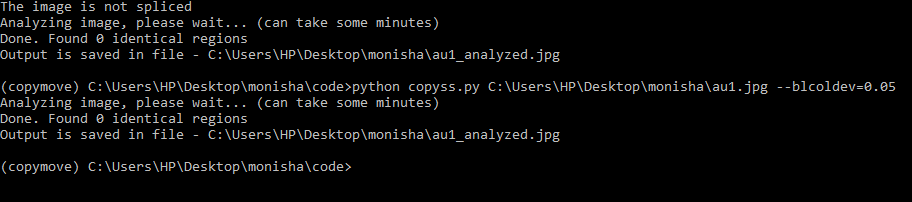
\includegraphics[width=15cm,height=4cm]{Figures/auth.PNG}
\caption{Output}
\label{fig:lion}
\end{figure}
\newpage
\subsection{TESTCASE 2}
\subsubsection{Spliced image}

\begin{figure}[htp]
\centering
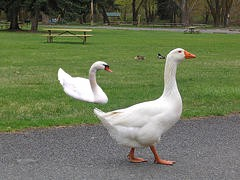
\includegraphics[width=10cm,height=7cm]{Figures/s1_resaved.jpg}
\caption{Spliced input image}
\label{fig:lion}
\end{figure}
\begin{figure}[htp]
\centering
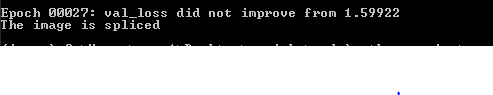
\includegraphics[width=15cm,height=5cm]{Figures/splicecmd.png}
\caption{Output}
\label{fig:lion}
\end{figure}
\newpage
\subsection{TESTCASE 3}
\subsubsection{Copy move}
\begin{figure}[htp]
\centering
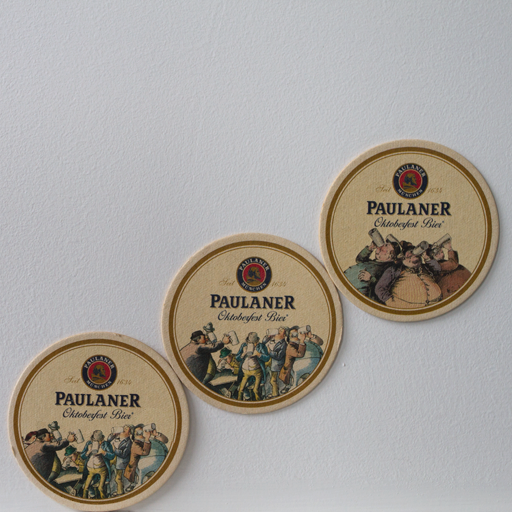
\includegraphics[width=7cm,height=6cm]{Figures/c1.png}
\caption{Copy move input image}
\label{fig:lion}
\end{figure}
\begin{figure}[htp]
\centering
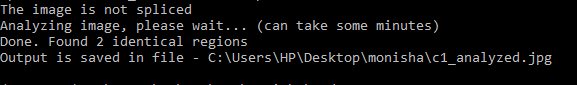
\includegraphics[width=15cm]{Figures/copycomd.PNG}
\caption{Output}
\label{fig:lion}
\end{figure}
\begin{figure}[htp]
\centering
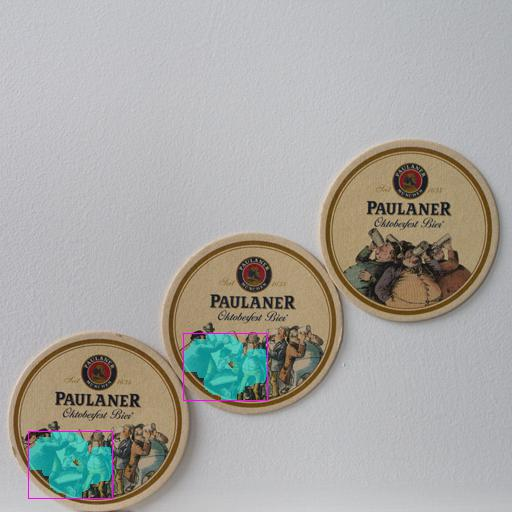
\includegraphics[width=7cm,height=6cm]{Figures/c1_analyzed.jpg}
\caption{Resaved image}
\label{fig:lion}
\end{figure}

